\documentclass[11pt]{article}
\usepackage{../cs70, latexsym,epsf,amsmath,amsfonts,graphicx,url}

% Space between paragraphs
\setlength{\parskip}{10pt plus 1pt minus 1pt}

\lecture{3}
\def\title{Note \the\lecturenumber}

\newcounter{thm}
\addtocounter{thm}{\the\lecturenumber}

\newtheorem{theorem}{Theorem}[thm]
\newtheorem{algorithm}{Algorithm}[thm]
\newtheorem{lemma}{Lemma}[thm]
\newtheorem{fact}{Fact}[thm]
\newtheorem{definition}{Definition}[thm]
\newtheorem{conjecture}{Conjecture}[thm]
\newtheorem{counterexample}{Counterexample}[thm]
\newtheorem{corollary}{Corollary}[thm]
\newtheorem{observation}{Observation}[thm]


\begin{document}
\maketitle

\section{Mathematical Induction}\label{scn:induction}

\paragraph{Introduction.} 
In this note, we introduce the proof technique of \emph{mathematical induction}. Induction is a powerful tool which is used to establish that a statement holds for \emph{all} natural numbers. Of course, there are infinitely many natural numbers --- induction provides a way to reason about them by finite means.

Let us demonstrate the intuition behind induction with an example. Suppose we wish to prove the statement: For all natural numbers $n$, $0 + 1 + 2 + 3 + \cdots + n = \frac{n(n+1)}{2}$. More formally, using the universal quantifier from Note 1, we can write this as:
\begin{equation}\label{eqn:1}
\forall n \in \N, \quad\sum^n_{i=0} i=\frac{n(n+1)}{2}.
\end{equation}
How would you prove this? Well, you could begin by checking that it holds for $n=0,1,2$, and so forth. But there are an {infinite} number of values of $n$ for which it needs to be checked! Moreover, checking just the first few values of $n$ does \emph{not} suffice to conclude the statement holds for all $n\in\N$, as the following example demonstrates:

\sanity{Consider the statement: $\forall n\in\N$, $n^2-n+41$ is a prime number. Check that it holds for the first few natural numbers. (In fact, you could check all the way up to $n=40$ and not find a counterexample!) Now check the case of $n=41$.}

In mathematical induction, we circumvent this problem by making an interesting observation: Suppose the statement holds for some value $n=k$, i.e. $\sum^k_{i=0} i=\frac{k(k+1)}{2}$. (This is called the \emph{induction hypothesis}.) Then:
\begin{equation}\label{eqn:2_1}
\left(\sum_{i=0}^{k} i\right) + (k+1)
= \frac{k(k+1)}{2} + (k+1)
= \frac{(k+1)(k+2)}{2},
\end{equation}
i.e. the claim must also hold for $n=k+1$! In other words, if the statement holds for some $k$, then it must also hold for $k+1$. Let us call the argument above the \emph{inductive step}. The inductive step is a very powerful tool: If we can show the statement holds for $k$, then the inductive step allows us to conclude that it also holds for $k+1$; but now that $k+1$ holds, the inductive step implies that $k+2$ must hold; in fact, we can repeat this argument indefinitely for all $n\geq k$! So is that it? Have we proven Equation~(\ref{eqn:1})? Almost!

The problem is that in order to apply the inductive step, we first have to establish that Equation~(\ref{eqn:1}) holds for some \emph{initial} value of $k$. Since our aim is to prove the statement for all natural numbers, the obvious choice is $k=0$. We call this choice of $k$ the \emph{base case}. Then, if the base case holds, the axiom of \emph{mathematical induction} says that the inductive step allows us to conclude that the Equation~{\ref{eqn:1}} indeed holds for all $n\in\N$.

Let us now formally re-write this proof.
\begin{theorem}
    $\forall n \in \N$, $\displaystyle\sum_{i=0}^n i = \frac{n(n+1)}{2}$.
\end{theorem}
\begin{proof}
We proceed by \emph{induction} on the variable $n$.

\emph{Base case $(n=0)$}: Here, we have $\displaystyle\sum_{i=0}^0 i = 0 = \frac{0(0+1)}{2}$. Thus, the base case is correct.

\emph{Inductive Hypothesis}: For arbitrary $n=k\geq 0$, assume that $\sum_{i=0}^k i = \frac{k(k+1)}{2}$. In words, the Inductive Hypothesis says ``let's assume we have proved the statement for an arbitrary value of $n =k \geq 0$''.

\emph{Inductive Step}: Prove the statement for $n=(k+1)$, i.e. show that $\sum_{i=0}^{k+1} i = \frac{(k+1)(k+2)}{2}$:
\begin{equation}\label{eqn:2}
\displaystyle\sum_{i=0}^{k+1} i = \left(\sum_{i=0}^{k} i\right) + (k+1)
= \frac{k(k+1)}{2} + (k+1)
= \frac{k(k+1)+ 2(k+1)}{2}
= \frac{(k+1)(k+2)}{2},
\end{equation}
where the second equality follows from the Induction Hypothesis. By the principle of mathematical induction, the claim follows.
\end{proof}

\sanity{How exactly did the Induction Hypothesis help us show the second equality in Equation~(\ref{eqn:2})? (Hint: We used it to replace $\sum_{i=0}^{k} i$ with something useful.)}

\paragraph{Recap.} What have we learned so far? Letting $P(n)$ denote the statement $\sum_{i=0}^{n} i = \frac{n(n+1)}{2}$, our goal was to prove that $\forall n \in \N$, $P(n)$. The {\em principle of induction}
asserts that to prove this requires three simple steps:
\begin{compactenum}
  \item \textbf{Base Case}: Prove that $P(0)$ is true.
  \item \textbf{Inductive Hypothesis}: For arbitrary $k\geq 0$, assume that $P(k)$ is true.
  \item \textbf{Inductive Step}: With the assumption of the Inductive Hypothesis in hand, show that $P(k+1)$ is true.
\end{compactenum}
Let us visualize how these three steps fit together using dominoes. Let statement $P(n)$ be represented by a sequence of dominoes, numbered from $0, 1, 2, ..., n$, such that $P(0)$ corresponds to the $0^{th}$ domino, $P(1)$ corresponds to the $1^{st}$ domino, and so on. The dominoes are lined up so that if the $k^{th}$ domino is knocked over, then it in turn knocks over the $k+1^{st}$.  Knocking over the $k^{th}$ domino corresponds to proving $P(k)$ is true. And the induction step corresponds to the placement of the dominoes to ensure that if the $k^{th}$ domino falls, in turn it knocks over the $k+1^{st}$ domino. The base case ($n=0$) knocks over the $0{th}$ domino, setting off a chain reaction that knocks down all the dominoes!

\begin{center}
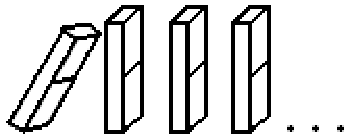
\includegraphics[scale = 0.7]{induction}
\end{center}

Finally, a word about choosing an appropriate base case --- in this example, we chose $k=0$, but in general, the choice of base case will naturally depend on the claim you wish to prove.

\paragraph{Another proof by induction.} Let us do another proof by induction. Recall from Note 1 that for integers $a$ and $b$, we say that $a$ \emph{divides} $b$, denoted $a|b$, if and only if there exists an integer $q$ satisfying $b = aq$.

\sanity{How would you write the definition of $a|b$ formally using quantifiers? (Answer: $\forall a$, $b \in \Z$, $a|b$ iff $\exists\; q \in \Z$ such that $b=aq$.)}

\begin{theorem} $\forall n \in \N$, $n^3 - n$ is divisible by 3.
\end{theorem}
\begin{proof}
We proceed by induction over $n$. Let $P(n)$ denote the statement $\forall n \in \N$,
$n^3 - n$ is divisible by 3.

\emph{Base case ($n=0$):} $P(0)$ asserts that $3|(0^3 - 0)$ or $3|0$, which is true since any non-zero integer divides $0$.

\emph{Inductive Hypothesis:} Assume for $n=k\geq 0$ that $P(k)$ is true. That is, $3|(k^3-k)$, or $\exists q \in \Z, k^3 - k = 3q$.

\emph{Inductive Step:} We show that $P(k+1)$ is true, i.e. that $3|((k+1)^3-(k+1))$. To show this, we expand the number $((k+1)^3-(k+1))$ as follows:
\begin{eqnarray*}
(k+1)^3 - (k+1) &=& k^3 + 3k^2 + 3k + 1 - (k+1) \\
&=& (k^3 - k) + 3k^2 + 3k \\
&=& 3q + 3(k^2 + k) \text{ for some }q \in \Z \quad\text{(Induction Hypothesis)}\\
&=& 3(q + k^2 + k).
\end{eqnarray*}

\sanity{How exactly did the Induction Hypothesis help us show the third equality above?}

\noindent We conclude that $3|((k+1)^3-(k+1))$. Thus, by the principle of induction, $\forall n \in \N$, $3|(n^3-n)$.
\end{proof}

\paragraph{Two Color Theorem.} We now consider a more advanced proof by induction for a simplified version of the famous \emph{four color theorem}. The four color theorem states that
any map can be colored with four colors such that any two adjacent countries (which share a border,
but {not} just a point) have different colors.  The four color theorem is very difficult to
prove, and several bogus proofs were claimed since the problem was first posed in 1852.
In fact, it was not until 1976 that a computer-assisted proof of the theorem was finally given Appel and Haken.  (For an interesting history of the problem and state-of-the-art proof, which is nonetheless still very challenging, see \url{www.math.gatech.edu/~thomas/FC/fourcolor.html}).

In this note, we consider a simpler version of the theorem in which our ``map'' is given by a rectangle which is divided into regions by drawing lines, such that each line divides the rectangle into two regions.  Can we color such a map using no more than two colors (say, red and blue) such that no two bordering regions have the same color? To illustrate, here is an example of a two-colored map:
\begin{center}
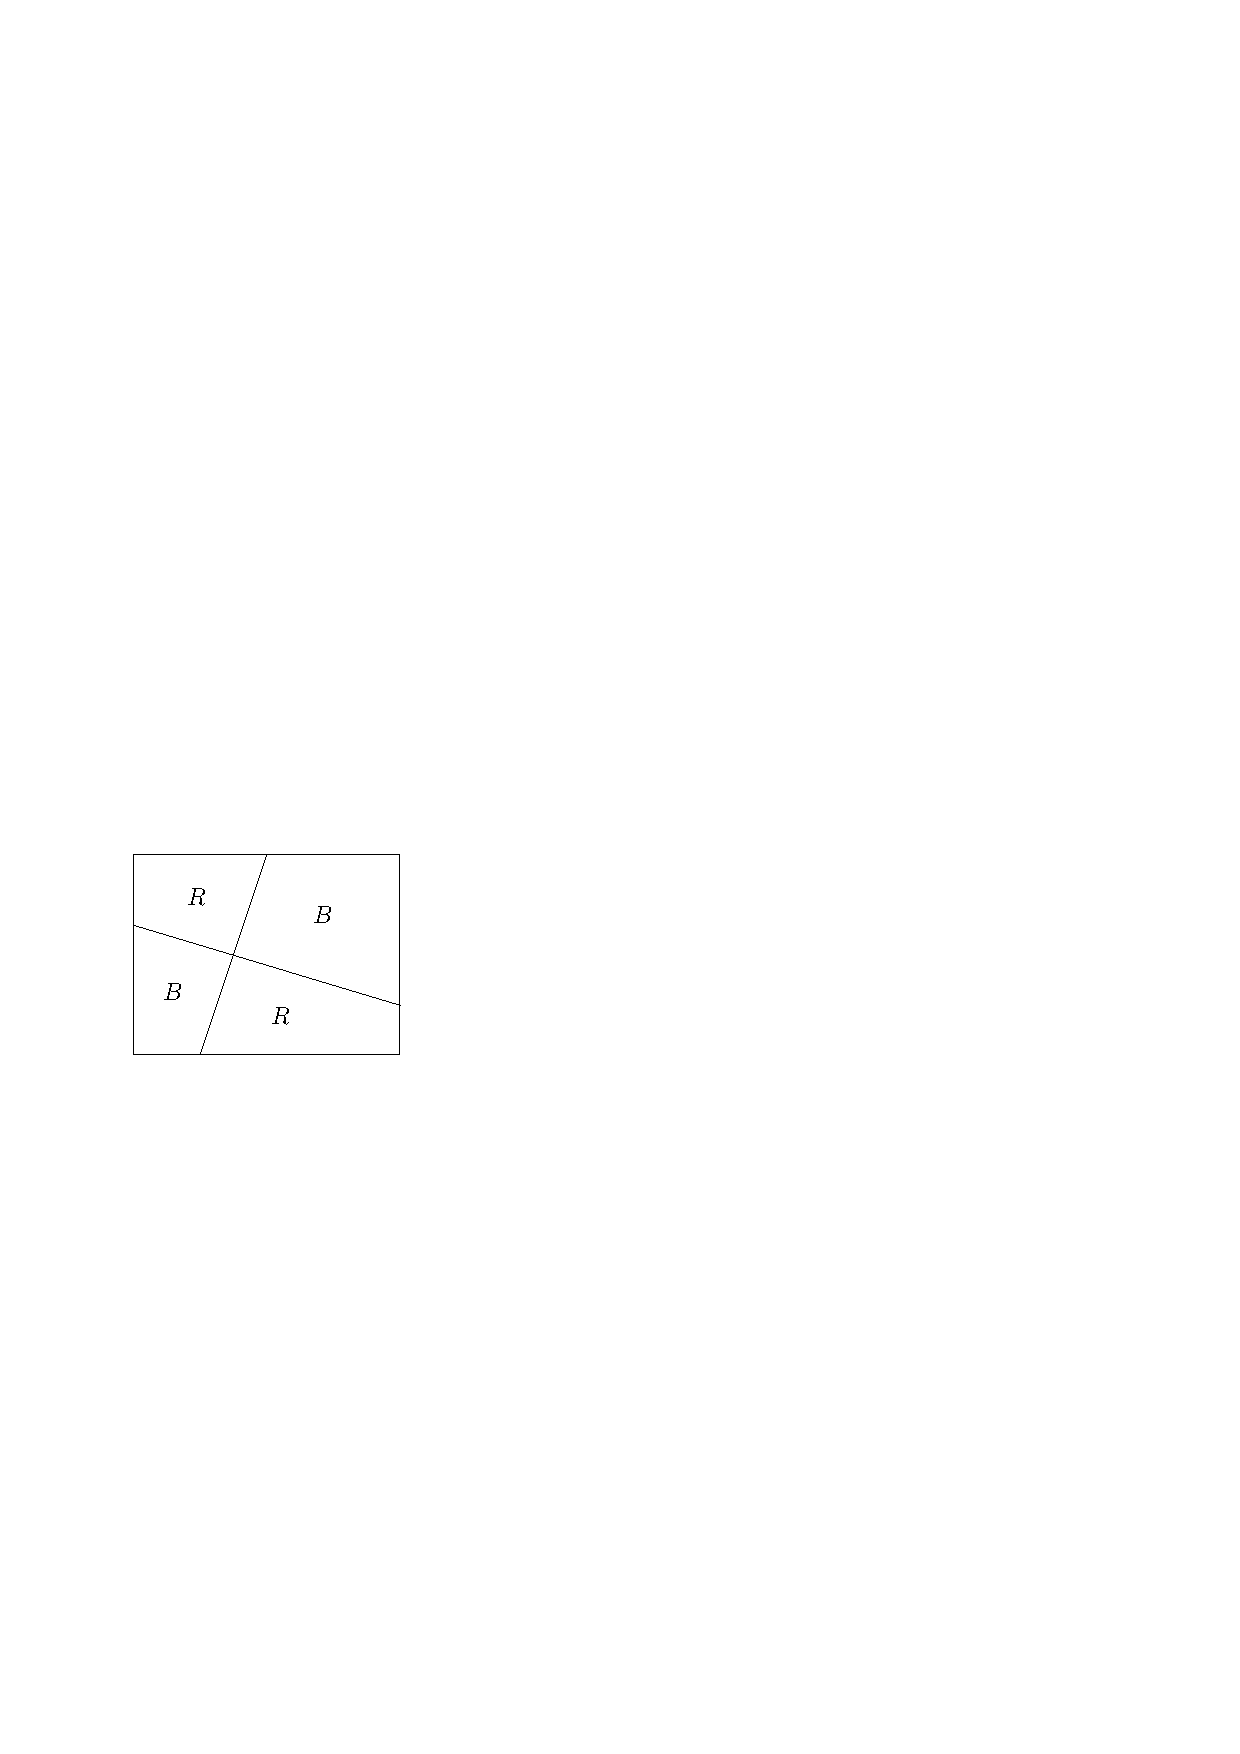
\includegraphics[scale = 0.9]{2color4}
\end{center}

\begin{theorem}\label{thm:2color}
    Let $P(n)$ denote the statement ``Any map with $n$ lines is two-colorable''. Then, it holds that $\forall n\in \N\; P(n)$.
\end{theorem}
\begin{proof}
We proceed by induction on $n$.

\emph{Base Case ($n=0$):} Clearly $P(0)$ holds, since if we have $n=0$ lines, then we can color
the entire map using a single color.

\emph{Inductive Hypothesis:} For any $n=k\geq 0$, assume $P(k)$.

\emph{Inductive Step:} We prove $P(k+1)$. Specifically, we are given a map with $k+1$ lines and wish to show
that it can be two-colored. Let's see what happens if we remove a line. With only $k$
lines on the map, the Induction Hypothesis says we can two-color the map. Let us make
the following observation: Given a valid coloring, if we swap red $\leftrightarrow$ blue, we still have a two-coloring.
With this in mind, let us place back the line we removed, and leave colors on one side of the line
unchanged. On the other side of the line, swap red $\leftrightarrow$ blue. This is illustrated by Figure~\ref{fig:map}. We claim that this is a valid two-coloring for the map with $k+1$ lines.\\

\begin{figure}[h]\label{fig:map}
\centering
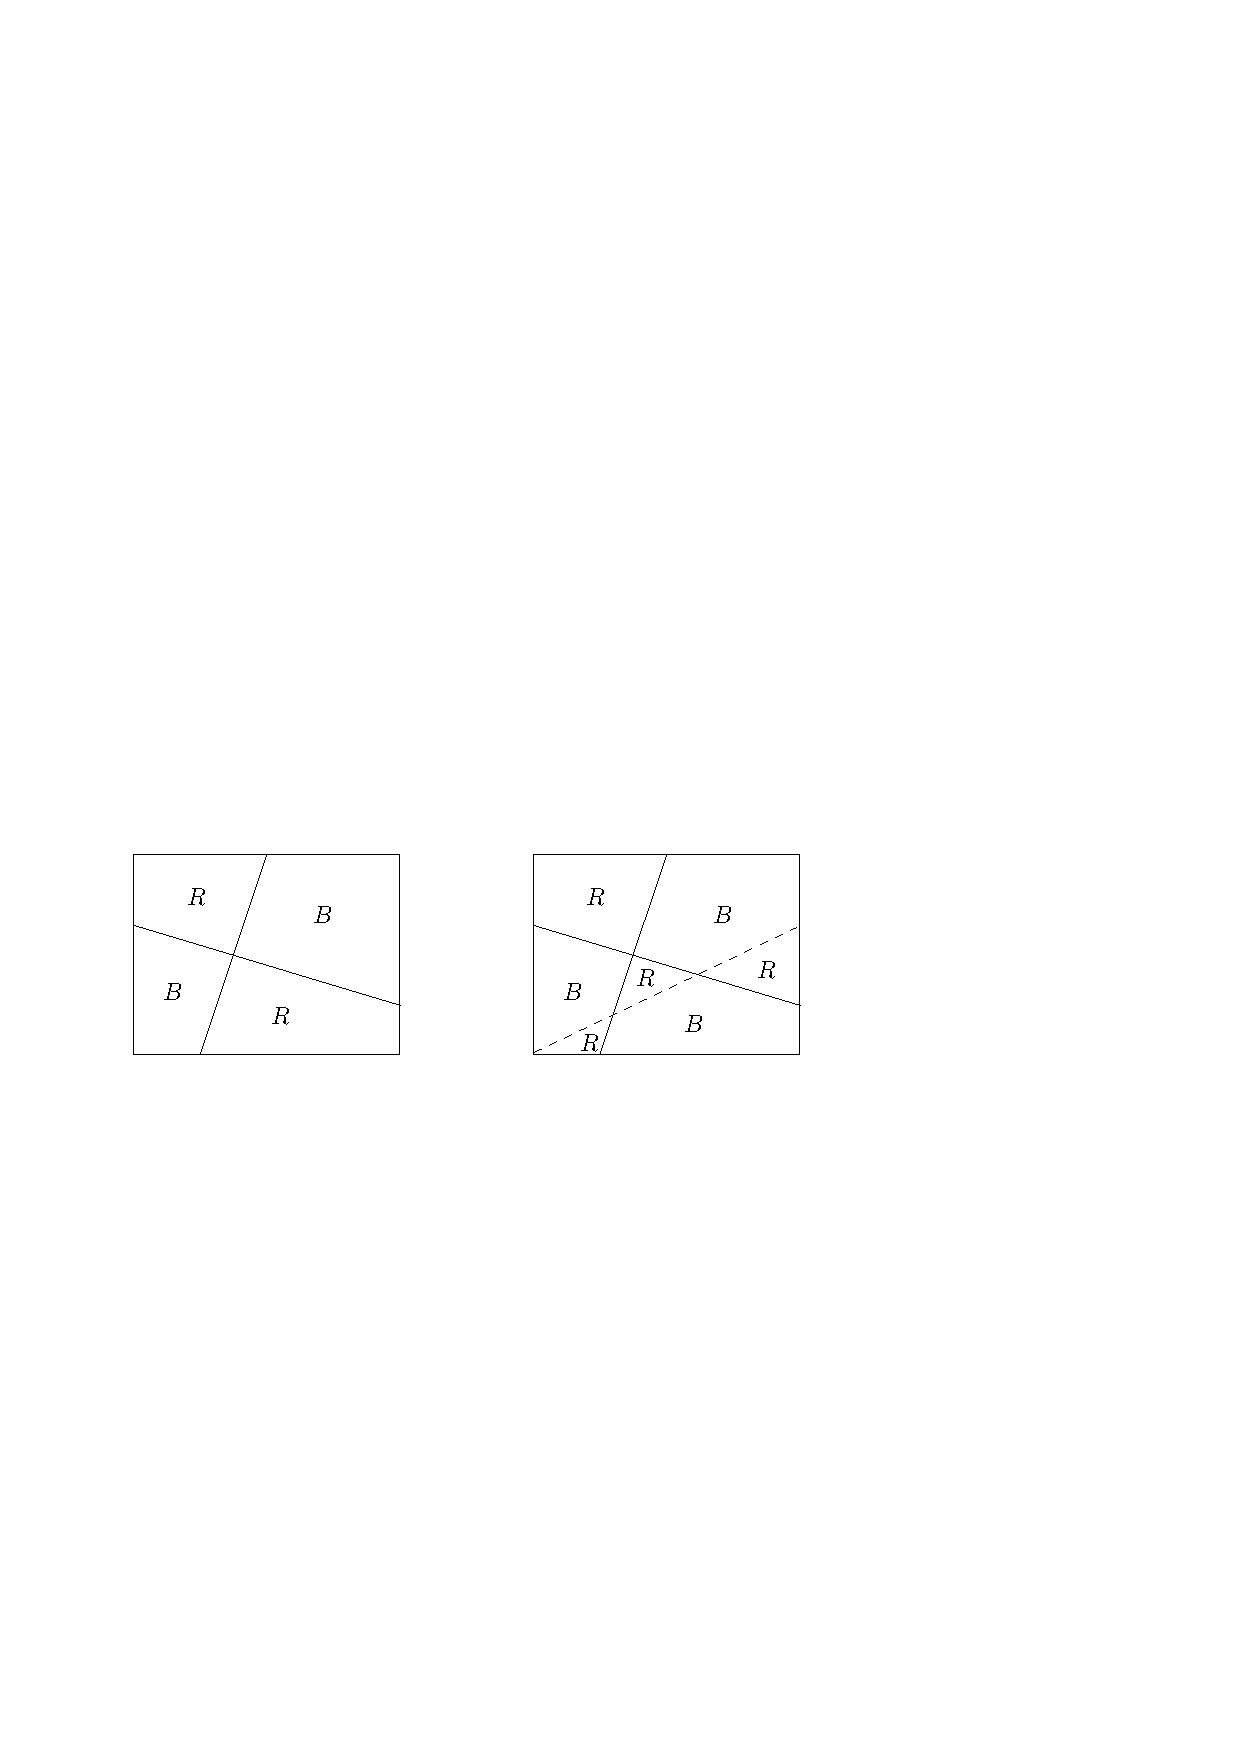
\includegraphics[scale = 0.8]{2color5}
\caption{(Left) The map with the $(k+1)$st line removed. (Right) The map with the $(k+1)$st line represented by dashed line.}
\centering
\end{figure}

Why does this work? Consider two regions separated by a shared border. Then, one of two cases must hold: Case 1 is when the shared border is the line that was removed and replaced, i.e. line $k+1$. But by construction, we flipped the colors on one side of this line so that any two regions separated by it have distinct colors. Case 2 is when the shared border is one of the original $k$ lines; here, the Induction Hypothesis guarantees that two regions separated by this border have different colors. Thus, in both cases, the regions separated by the shared border have distinct colors, as required.
\end{proof}

\section{Strengthening the Induction Hypothesis}

When using induction, it can be very important to choose the correct statement to prove. For example, suppose we wish to prove the statement: $\forall n \geq 1$, the sum of the first $n$ odd numbers is a perfect square. Here is a first proof attempt via induction.

\emph{Proof attempt.} We proceed by induction on $n$.

\emph{Base Case ($n = 1$):} The first odd number is $1$, which is a perfect square.

\emph{Inductive Hypothesis:} Assume that the sum of the first $k$
odd numbers is a perfect square, say $m^2$.

\emph{Inductive Step:} The $(k+1)$st odd number is $2k+1$. Thus, by the induction hypothesis, the sum of the first $k+1$ odd numbers is $m^2 + 2k +1$. But now we are stuck. Why should $m^2 + 2k+1$ be a perfect square? It seems our Induction Hypothesis is too ``weak''; it does not give us enough structure to say anything meaningful about the $(k+1)$ case.

So let's take a step back for a moment, and do a preliminary check to ensure our claim isn't obviously false: Let's compute the values of the first few cases. Perhaps in the process, we can also uncover some hidden structure we have not yet identified.
\begin{compactitem}
\item $n = 1: 1 = 1^2$ is a perfect square.
\item $n = 2: 1 + 3 = 4 = 2^2$ is a perfect square.
\item $n = 3: 1 + 3 + 5 = 9 = 3^2$ is a perfect square.
\item $n = 4: 1 + 3 + 5 + 7 = 16 = 4^2$ is a perfect square.
\end{compactitem}
It looks like we have good news and even better news: The good news is that we have not yet found a counterexample to our claim. The even better news is that there is a surprising pattern emerging --- the sum of the first $n$ odd numbers is not just a perfect square, but is equal precisely to $n^2$! Motivated by this discovery, let's try something counterintuitive: Let us try to show the following \emph{stronger} claim.

\begin{theorem}\label{thm:sumodd}
    For all $n \geq 1$, the sum of the first $n$ odd numbers is $n^2$.
\end{theorem}
\begin{proof}
We proceed by induction on $n$.

\emph{Base Case ($n = 1$):} The first odd number is $1$, which is $1^2$.

\emph{Inductive Hypothesis:} Assume that the sum of the first $k$
odd numbers is $k^2$.

\emph{Inductive Step:} The $(k+1)$-st odd number is $2k+1$. Applying the Induction Hypothesis, the sum of the first $k+1$ odd numbers is $k^2 + (2k +1) = (k+1)^2$. Thus, by the principle of induction the theorem holds.
\end{proof}

So let's get this straight --- we couldn't prove our original statement, so instead we hypothesized a stronger one and managed to prove that. Why on Earth did this work? The reason is that our original claim did not capture the true \emph{structure} of the underlying fact we were trying to prove --- it was too vague. As a result, our Induction Hypothesis wasn't strong enough to prove our desired result. In contrast, although our second claim is \emph{a priori} stronger, it also has more structure to it; this, in turn, makes our Induction Hypothesis stronger --- we can use the fact that not only is the sum of the first $k$ odd numbers a perfect square, but that it in fact equals $k^2$. This additional structure is exactly what we needed to complete the proof. In summary, we have demonstrated an example in which, although a claim was true, the precise formulation of the Induction Hypothesis made the difference between a failing and successful proof.

\paragraph{Example.} Let us now try a second example; this time, we'll let you do some of the work! Suppose we wish to prove the claim: $\forall n \geq 1$, $\sum_{i=1}^n \frac{1}{i^2}\leq 2$.\\

\sanity{The ``obvious'' choice of Induction Hypothesis says the following: Assume that for $n=k$,
    $\sum_{i=1}^k \frac{1}{i^2}\leq 2$. Why does this not suffice to prove the claim for $n=k+1$, i.e. to show that $\sum_{i=1}^k \frac{1}{i^2} + \frac{1}{(i+1)^2}\leq 2$? (Hint: Is it possible that $\sum_{i=1}^k \frac{1}{i^2}$ actually \emph{equals} $2$?)}

Now let's again do the unthinkable --- let's prove the following \emph{stronger} statement, i.e. let's strengthen our induction hypothesis.

\begin{theorem}\label{thm:sumlessthan2}
    For all $n \geq 1$, $\displaystyle\sum_{i=1}^n \frac{1}{i^2}\leq 2-\frac{1}{n}$.
\end{theorem}
\begin{proof}
We proceed by induction on $n$.

\emph{Base Case ($n = 1$):} We have $\displaystyle\sum_{i=1}^1\frac{1}{i^2}=1\leq 2-\frac{1}{1}$, as required.

\emph{Inductive Hypothesis:} Assume that the claim holds for $n=k$.

\emph{Inductive Step:} By the Induction Hypothesis, we have that
\[
    \sum_{i=1}^{k+1} \frac{1}{i^2}=\sum_{i=1}^{k} \frac{1}{i^2}+ \frac{1}{(k+1)^2}\leq 2-\frac{1}{k} + \frac{1}{(k+1)^2}.
\]
Thus, to prove our claim, it suffices to show that
\begin{equation}\label{eqn:bound}
    -\frac{1}{k} + \frac{1}{(k+1)^2} \leq -\frac{1}{k+1}.
\end{equation}

\exercise{Show that Equation~(\ref{eqn:bound}) holds. (Hint: Multiply both sides of the inequality by $(k+1)$.)}

By the principle of mathematical induction, the claim holds.
\end{proof}



\section{Simple Induction vs. Strong Induction}

Thus far, we have been using a notion of induction known as \emph{simple} or \emph{weak} induction. There is another notion of induction, which we now discuss, called \emph{strong} induction. The latter is similar to simple induction, except we have a slightly different inductive hypothesis: Instead of just assuming $P(k)$ is true (as was the case with simple induction), we assume the stronger statement that $P(0)$, $P(1)$, \ldots, and $P(k)$ are \emph{all} true (i.e. that $\bigwedge_{i=0}^{k} P(i)$ is true).

Is there a difference between the power of strong and weak induction, i.e. can strong induction prove statements which weak induction cannot? \emph{No!} Intuitively, this can be seen by returning to our domino analogy from Section~\ref{scn:induction}. In this picture, weak induction says that if the $k$th domino falls, so does the $(k+1)$st one, whereas strong induction says that if dominos $1$ through $k$ fall, then so does the $(k+1)$st one. But these scenarios are equivalent: If the first domino falls, then applying weak induction repeatedly we conclude that the first domino in turn topples dominos $2$ through $k$, setting up the case of $k+1$, just as is the case with strong induction. With that said, strong induction does have an appealing advantage --- it can make proofs \emph{easier}, since we get to assume a stronger
hypothesis. How should we understand this? Consider the analogy of a screwdriver and a power screwdriver --- they both accomplish the same task, but the latter is much easier to use!

Let's try a simple example\footnote{This problem also goes under the name of the Postage Stamp Problem, which states that every amount of postage over $12$ cents can be paid using $4$- and $5$-cent stamps.} of strong induction. As a bonus, this is our first induction proof requiring \emph{multiple} base cases.
\begin{theorem}\label{thm:sumeven}
    For every natural number $n\geq 12$, it holds that $n=4x+5y$ for some $x,y\in\N$.
\end{theorem}
\begin{proof}
We proceed by induction on $n$.

\emph{Base Case ($n = 12$):} We have $12=4\cdot 3+5\cdot 0$.

\emph{Base Case ($n = 13$):} We have $13=4\cdot 2+5\cdot 1$.

\emph{Base Case ($n = 14$):} We have $14=4\cdot 1+5\cdot 2$.

\emph{Base Case ($n = 15$):} We have $15=4\cdot 0+5\cdot 3$.

\emph{Inductive Hypothesis:} Assume that the claim holds for all $12\leq n\leq k$ for $k\geq 15$.

\emph{Inductive Step:} We prove the claim for $n=k+1\geq 16$. Specifically, note that $(k+1)-4\geq 12$; thus, the Induction Hypothesis implies that $(k+1)-4=4x'+5y'$ for some $x',y'\in\N$. Setting $x=x'+1$ and $y=y'$ completes the proof.
\end{proof}
\sanity{Why would the proof above fail if we used weak induction instead of strong induction?}

Let's try a second, more advanced, example. For this, recall that a number $n\geq 2$ is prime if $1$ and $n$ are its only divisors.

\begin{theorem}\label{thm:prodprimes}
    Every natural number $n > 1$ can be written as a product of primes.
\end{theorem}
\begin{proof}
We proceed by induction on $n$. Let $P(n)$ be the proposition
that $n$ can be written as a product of primes. We will prove that $P(n)$ is true for all $n \geq 2$.

\emph{Base Case ($n=2$):} We start at $n = 2$. Clearly $P(2)$ holds, since 2 is a prime number.

\emph{Inductive Hypothesis:} Assume $P(n)$ is true \emph{for all} $2 \leq n \leq k$.

\emph{Inductive Step:} Prove that $n=k+1$ can be written as a product of primes.
We have two cases: either $k+1$ is a prime number, or it is not.  For the first case, if $k+1$ is a prime
number, then we are done. For the second case, if $k+1$ is not a prime number, then by definition $k+1 = xy$ for some $x$,$y \in \Z^+$ satisfying $1 < x,y < k+1$. By the Induction Hypothesis, $x$ and $y$ can each be written as a product of primes
(since $x,y \leq n$). But this implies that $k+1$ can also be written as a product of primes.
\end{proof}

\sanity{Why does this proof fail if we instead use simple induction? (Hint: Suppose $k=42$. Since $42=6\times 7$, in the Inductive Step we wish to use the facts that $P(6)$ and $P(7)$ are true. But weak induction does not give us this --- which value of $P$ does weak induction allow us to assume is true in this case?)}

Finally, for those who wish to have a more formal understanding of why weak and strong induction are equivalent, consider the following. Let $Q(n)=P(0)\wedge P(1)\wedge\cdots\wedge P(n)$. Then, strong induction on $P$ is equivalent to weak induction on $Q$.



\section{Recursion, programming, and induction}

There is an intimate connection between induction and recursion, which we explore here via two examples.

\paragraph{Example 1: Fibonacci's rabbits.} In the 13th century lived a famous Italian mathematician known as \emph{Fibonacci}\footnote{Fibonacci was also known as Leonardo of Pisa. If you ever find yourself in Pisa, Italy, you can visit his grave; his remains are buried at Campo Santo.}, who in 1202 considered the following rabbit-based puzzle: Starting with a pair of rabbits, how many rabbits are there after a year, if each month each pair begets a new pair which from the second month on becomes productive? This model of population growth can be modeled by recursively defining a function; the resulting sequence of numbers is nowadays referred to as the \emph{Fibonacci} numbers.

To recursively model our rabbit population, let $F(n)$ denote the number of pairs of rabbits in month $n$.  By the rules above, our initial conditions are as follows: Clearly $F(0)=0$. In month $1$, a single pair of rabbits is introduced, implying $F(1) = 1$. Finally, since it takes a month for new rabbits to become reproductive, we also have $F(2) = 1$.

In month $3$, the fun begins. For example, $F(3)=2$, since the original pair breeds to produce a new pair. But how about $F(n)$ for a general value of $n$? It seems difficult to give an explicit formula for $F(n)$. However, we can define $F(n)$ \emph{recursively} as follows. In month $n -1$, by definition we have $F(n-1)$ pairs. How many of these pairs were productive? Well, only those that were already alive in the previous month, i.e. $F(n-2)$ of them. Thus, we have $F(n-2)$ new pairs in the $n$th month in addition to our existing $F(n-1)$ pairs. Hence, we have $F(n) = F(n-1) + F(n-2)$. To summarize:
\begin{compactitem}
	\item $F(0) = 0$.
    \item $F(1) = 1$.
	\item For $n \geq 2$, $F(n) = F(n-1) + F(n-2)$.
\end{compactitem}
Pretty neat, except you might wonder why we care about rabbit reproduction in the first place! It turns out this simplified model of population growth illustrates a fundamental principle: Left unchecked, populations grow exponentially over time. 
In fact, understanding the significance of this unchecked exponential population growth
was a key step that led Darwin to formulate his theory of evolution.
To quote Darwin: ``There is no exception to the rule that every organic being
increases at so high a rate, that if not destroyed, the earth would soon be
covered by the progeny of a single pair."


Now, we promised you programming in the title of this section, so here it is --- a trivial recursive program to evaluate $F(n)$:
\noindent
\begin{tabbing}
\quad\={\tt function F(n)}\\
\>\quad\=	{\tt if n=0 then return 0}\\	
\>\>		{\tt if n=1 then return 1}\\
\>\>		{\tt else return F(n-1) + F(n-2)}
\end{tabbing}			

\exercise{How long does it take this program to compute $F(n)$, i.e. how many calls to $F(n)$ are needed?}

The exercise above should convince you that this is a very inefficient way to compute the $n$th Fibonacci number. Here is a much faster iterative algorithm to accomplish the same task (this should be a familiar example of turning a tail-recursion into an iterative
algorithm):

\noindent
\begin{tabbing}
\quad\={\tt function $\hbox{\tt F}_2$(n)}\\
\>\quad\=	{\tt if n=0 then return 0}\\	
\>\>		{\tt if n=1 then return 1}\\
\>\>		{\tt a = 1}\\
\>\>		{\tt b = 0}\\
\>\>		{\tt for k = 2 to n do}\\
\>\>\quad\=	{\tt temp = a}\\
\>\>\>		{\tt a = a + b}\\
\>\>\>		{\tt b = temp}\\
\>\>		{\tt return a}
\end{tabbing}
			
  \exercise{How long does this iterative algorithm take to compute $F_2(n)$, i.e. how many iterations of its loop are needed? Can you show by induction that this new function $F_2(n) = F(n)$?}

\paragraph{Example 2: Binary search.} We next use induction to analyze a recursive algorithm which even your grandmother is likely familiar with --- binary search! Let us discuss binary search in the context of finding a word in the dictionary: To find word $W$, we open the dictionary to its middle page. If the letter of that page comes after the first letter of $W$, we recurse on the first half of the dictionary; else, we recurse on the last half of the dictionary. (For simplicity, we ignore the issue of dividing a dictionary with an \emph{odd} number of pages into two halves.) Once we've narrowed down the dictionary to a single page, we resort to a brute force search to find $W$ on that page. In pseudocode, we have:
\begin{compactenum}
            \item //precondition:  $W$ is a word and $D$ is a subset of the dictionary with at least $1$ page.
            \item //postcondition: Either the definition of $W$ is returned, or ``$W$ not found'' is returned.
            \item findWord($W$, $D$) \{
            \item \mbox{\hspace{5mm}} //Base case
            \item \mbox{\hspace{5mm}} If ($D$ has precisely one page)
            \item \mbox{\hspace{10mm}} Look for $W$ in $D$ by brute force. If found, return its definition; else, return ``$W$ not found''.
            \item
            \item \mbox{\hspace{5mm}} //Recursive case
            \item \mbox{\hspace{5mm}} Let $W'$ be the first word on the middle page of $D$.
            \item \mbox{\hspace{5mm}} If ( $W$ comes before $W'$ )
            \item \mbox{\hspace{10mm}}return findWord( first half of $D$ )
            \item \mbox{\hspace{5mm}} Else
            \item \mbox{\hspace{10mm}}return findWord( last half of $D$ )
            \item \}
\end{compactenum}

Let us prove using induction that findWord() is \emph{correct}, i.e. it returns the definition of $W$ if $W$ is in the dictionary $D$. As a bonus, the proof requires us to use \emph{strong} induction instead of simple induction!

\begin{proof}[Proof of correctness of findWord().]
    We proceed by strong induction on the number of pages, $n$, in $D$.

\emph{Base Case ($n = 1$):} If $D$ has one page, line $6$ searches via brute force for $W$. Thus, if $W$ is present, it is found and returned; else, we return ``$W$ not found'', as desired.

\emph{Inductive Hypothesis:} Assume that findWord() is correct for all $1\leq n\leq k$. We prove it is correct for $n=k+1$.

\emph{Inductive Step:} After Step 9, we know $W'$; thus we can determine whether $W$ must be in  the first or second half of $D$. In the first case, we recurse on the first half of $D$ in line 11, and in the second case we recurse on the second half of $D$ in line 13. By the Induction Hypothesis, the recursive call correctly finds $W$ in the first or second half, or returns ``$W$ not found''. Since we return the recursive call's answer, we conclude that findWord() correctly finds $W$ in $D$ of size $n=k+1$. By the principle of mathematical induction, the findWord() is correct.
\end{proof}

\sanity{Why did we require \emph{strong} induction in the proof above?}

\section{False proofs}

It is very easy to prove false things if your proof is incorrect! Let's illustrate with a famous example. In the middle of the last century, a colloquial expression in common use was ``that is a horse of a different color", referring to something that is quite different
from normal or common expectation. The reknowned mathematician George Polya, who was also a
great expositor of mathematics for the lay public, gave the following proof
to show that there is no horse of a different color!

\begin{theorem} \label{thm:horses}
All horses are the same color.
\end{theorem}
\begin{proof}
We proceed by induction on the number of horses, $n$. Let $P(n)$ denote the statement of the claim.

\emph{Base Case ($n=1$):} $P(1)$ is certainly true, since if you have a set containing just
one horse, all horses in the set have the same color.

\emph{Inductive Hypothesis:} Assume $P(n)$ holds for any $n\geq 1$.

\emph{Inductive Step:} Given a set of $n+1$ horses $\{h_1,h_2,\ldots,h_{n+1}\}$,
we can exclude the last horse in the set and apply the inductive hypothesis
just to the first $n$ horses $\{h_1,\ldots,h_n\}$, deducing that they all have
the same color. Similarly, we can conclude that the last $n$ horses $\{h_2,\ldots,h_{n+1}\}$
all have the same color. But now the ``middle'' horses $\{h_2,\ldots,h_n\}$ (i.e., all
but the first and the last) belong to both of these sets, so they have the same
color as horse~$h_1$ and horse~$h_{n+1}$.  It follows, therefore, that all $n+1$ horses
have the same color. We conclude, by the principle of induction, that all horses have the same color.
\end{proof}

Clearly, it is not true that all horses are of the same color! So, where did we go wrong? Recall that in order for the principle of mathematical induction to apply, the induction step must show the statement: $\forall n\geq 1$, $P(n)\lra P(n+1)$. We claim that in the proof above, this statement is false --- in particular, there exists a choice of $n$ which yields a \emph{counterexample} to this statement.

\exercise{For which value of $n$ is it \emph{not} true that $P(n)\lra P(n+1)$? (Hint: Think about the key property in the proof of having ``middle'' horses.)}


\section{Practice Problems}

\begin{enumerate}

\item Prove for any natural number $n$ that $1^2 + 2^2 + 3^2 + \ldots + n^2 = \frac{1}{6}n(n+1)(2n+1)$.

\item Prove that $3^n > 2^n$ for all natural numbers $n \geq 1$.

\item In real analysis, Bernoulli's Inequality is an inequality which approximates the exponentiations of $1+x$.
Prove this inequality, which states that $(1+x)^n \geq 1+nx$ if $n$ is a natural number and $1+x > 0$.


\item A common recursively defined function is the \emph{factorial}, defined for a nonnegative number $n$ as $n! = n(n-1)(n-2)...1$, with base case $0! = 1$. Let us reinforce our understanding of the connection between recursion and induction by considering the following theorem involving factorials.


{\bf Theorem: } $\forall n \in \N$, $n > 1 \Longrightarrow n! < n^n$.

Prove this theorem using induction. (Hint: In the Inductive Step, write $(n+1)!=(n+1)\cdot n!$, and use the Induction Hypothesis.)

\item A \emph{celebrity} at a party is someone whom everyone knows, yet who knows no
one.  Suppose that you are at a party with $n$ people.  For any pair of people
$A$ and $B$ at the party, you can ask $A$ if they know $B$ and receive an honest
answer.  Give a recursive algorithm to determine whether there is a celebrity at
the party, and if so who, by asking at most $3n - 4$ questions. (Note: for the
purpose of this question you are just visiting the party to ask questions. What
you are trying to determine is whether the $n$ people actually attending the
party include a celebrity).

Prove by induction that your algorithm always correctly identifies a celebrity
iff there is one, and that the number of questions is at most $3n-4$.

\end{enumerate}
\end{document}
